

\begin{frame}{Motivaci\'on}
    \begin{columns}[T]
        \begin{column}{0.48\linewidth}
            \centering
            \begin{tikzpicture}
                \node[inner sep=0pt] at (1.4,5.8) {
                    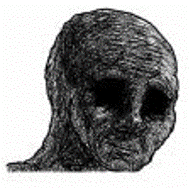
\includegraphics[width=2cm]{img/sface.png}
                };
        
        
                \node[inner sep=0pt] at (1.4,3.2) {
                    
\includegraphics[width=2cm]{img/hface.png}
                };
        
                \draw[-,thick] (0.3, 4.6) -- (6,4.5);
                \draw[-,thick] (2.7, 2) -- (2.7,6.8);
        
                \node[inner sep=0pt] at (4.4, 3.2) {
                    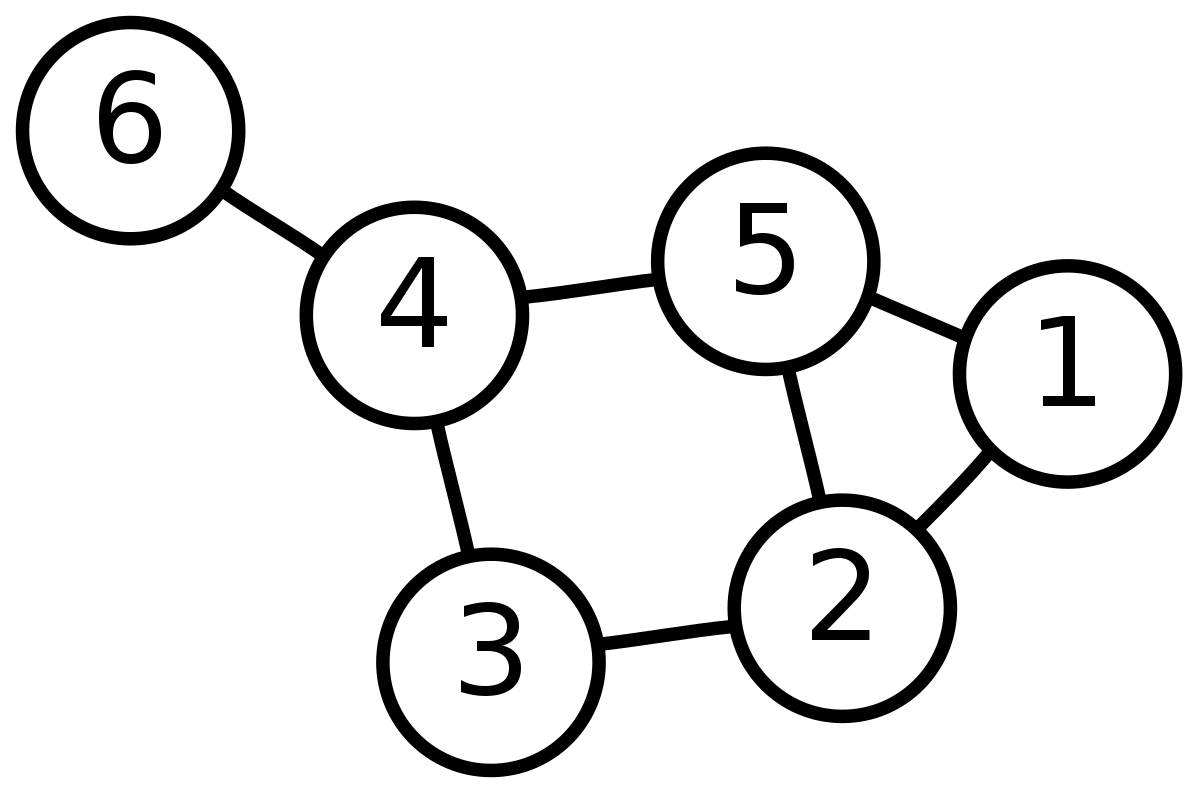
\includegraphics[width=3cm, height=2.5cm]{img/graph.png}
                };

                \node[align=left] at (5, 5.8) {\tiny $G=(V,A)$\\ \tiny $V:$ Conjunto finito de v\'ertices\\ \tiny $A:$ Conjunto de aristas $\{v,w\} : v,w \in V$} ;
        
            \end{tikzpicture}
        \end{column}

        \begin{column}{0.48\linewidth}
            \vspace{15mm}
            Las representaciones visuales permiten que los \textcolor{red}{conceptos} matem\'aticos y
            computacionales abstractos se vuelvan m\'as concretos
        \end{column}
        
    \end{columns}
   
\end{frame}

\begin{frame}{Concepto de base de datos}
    \begin{block}{}
        \begin{quote}
            ``... una base de datos es una colecci\'on auto-descriptiva de registros integrados."
            \hspace{1em plus 1fill}---Allen Taylor
        \end{quote}
    \end{block}

    \note{@NOTE \'enfasis en q lo que se registran son los datos y sus interrelaciones}
\end{frame}

\begin{frame}{¿Y si nos enfocamos en la idea?}

    \onslide<1->{
        \begin{block}{}
            \begin{itemize}
                \item Una base de datos es una colecci\'on de {\color<2>{red}conjuntos de registros} con la {\color<2>{red}misma estructura} entre los que se establecen {\color<2>{red}interrelaciones}.
            \end{itemize}
        \end{block}
    }

    \onslide<2->{
        \begin{alertblock}{Elementos principales}
            \begin{itemize}
                \item Conjuntos de registros
                \item Interrelaciones entre los conjuntos de registros
                \item Estructura de los registros
            \end{itemize}
        \end{alertblock}
    }
\end{frame}